\chapter{Designs}

\section{Class Structure}
\subsubsection{Effect Class Diagram}

\begin{center}
	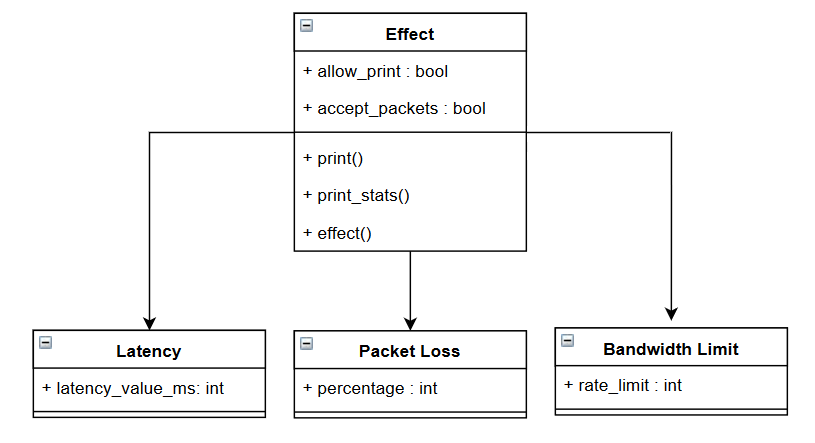
\includegraphics[scale=0.7]{Effect_Class_Design}
	\begin{figure}[h]
		\caption{UML Class diagram for producing degradation effects}
	\end{figure}
\end{center}

The above design is for the various effects that will be implemented into the program. They will be self contained within separate modules encased in an object. This was chosen so each effect is modular and self contained from one another, this will improve the potential readability and maintainability of the code base, it will also make the code base much more scalable where effects can be added with high speed because of the lack repeated code.  Each effect will inherit from the base class ``Effect", where it will obtain method and properties used for functionality, boolean variables for allowing printing and accepting packets, these are both necessary when `chaining' effects together, where a packet can only be accepted once and a single print will be required.

\subsubsection{Degradation effect Activity Diagram}

\begin{center}
	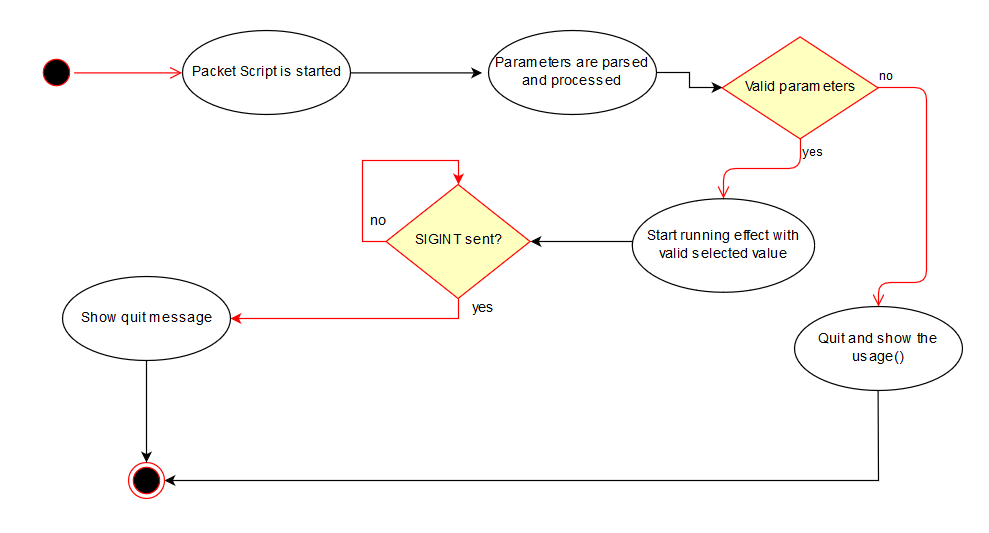
\includegraphics[scale=0.6]{Packet_Activity_Diagram}
	\begin{figure}[h]
		\caption{Activity Diagram for the degradation script}
	\end{figure}
\end{center}

Above is the activity diagram for the packet script that will implement the effect classes above, this script will be utilised directly from the command line or run by the GUI. The decision of having a single script that is controlled from multiple ways allow for one central point of functionality and means code can be shared throughout the project. The activity diagram shows the design choices for the direct control on the script. SIGINT is mentioned in the centre of the diagram, SIGINT is a built in signal in the Linux operating system that represents an interrupt signal, where it is triggered by pressing ``Control + C", this is the most common/clean way of stopping a script. The other alternatives to closing the script ``Control + Z" (SIGTSTP) and ``Control + /" (SIGQUIT) will be remapped to send a SIGINT signal and perform the same role, this will mean the program has one tidy point of closure.

\section{UI Design}
\subsection{Degradation effect User Interface}
One of the ways mentioned before to control the degradation effects is by a user interface. It needs to have a way to easily add new buttons and text entries that link up to parameters in the script to make the interface scalable and easy to maintain, It also needs a window to display the same output as the terminal window, this can be achieved by `piping' the stdout to a custom section of the user interface. The `stdout' is the data stream that links up to a Linux terminal window, if the stdout points to somewhere else it will display where it is needed. Below is the initial drafted design for the user interface.

\begin{center}
	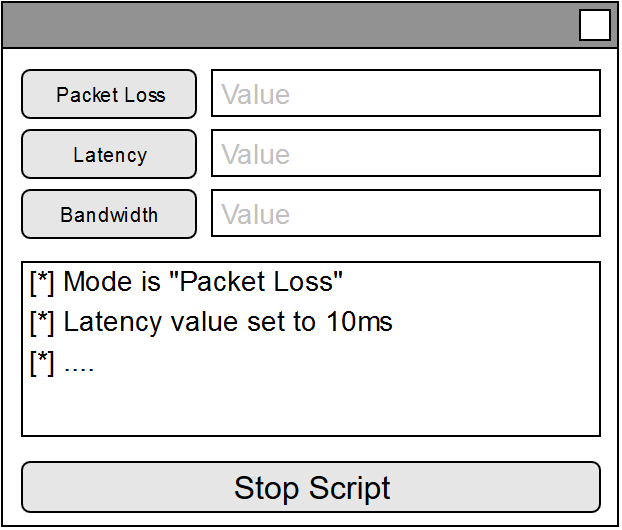
\includegraphics[scale=0.5]{Packet_UI_Design}
	\begin{figure}[h]
		\caption{Initial user interface design for the Degradation GUI}
	\end{figure}
\end{center}

Appendix A also contains the initial designs for the server client pairs.

\subsection{Deviations from initial designs}
The HTTP demonstration was intended to be a custom made client and server that sent custom HTTP requests that will perform some sort of trivial function. This was removed from the project and the replacement was to use 3 different modern browsers 
to request a web page. This gives the benefits of a more accurate real-world application along side of a complex function of the protocol. The demonstration will involve the loading of various websites while the degradation effects are active to see how quickly the web-page loads. As a related side and on line speed test will be run to display ping (latency) and the download and upload rate of the connection, this will give a intuitive metric that can be used to compare the effects of the degradation.

FTP also had reductions in its implementation. Initially it was intended to include a client and server pair. The client having various features is crucial for the demoing purposes, features including displaying accurate download rates and being and able to clearly view the servers contents. This functionality would take time to implement and a custom solution would not have added anything to the intended purpose of the project, this is why an open source solution FileZilla \footnote{\url{https://filezilla-project.org/}} was chosen as the solution with the required features being present.

\section{Experimental Design}
In the initial stages of the project there were experiments that tested the effects of the degradation on the network, the tests were performed on the loopback (Internal network 127.0.0.1) with ICMP ping packets.

%Latency graph
Latency was tested and graphed to see how each packet was affected by the test script, the latency parameter was 10 ms with 1000 packets sent in total. Each point of the graph is the latency of the ping value for a single packet.

\begin{center}
	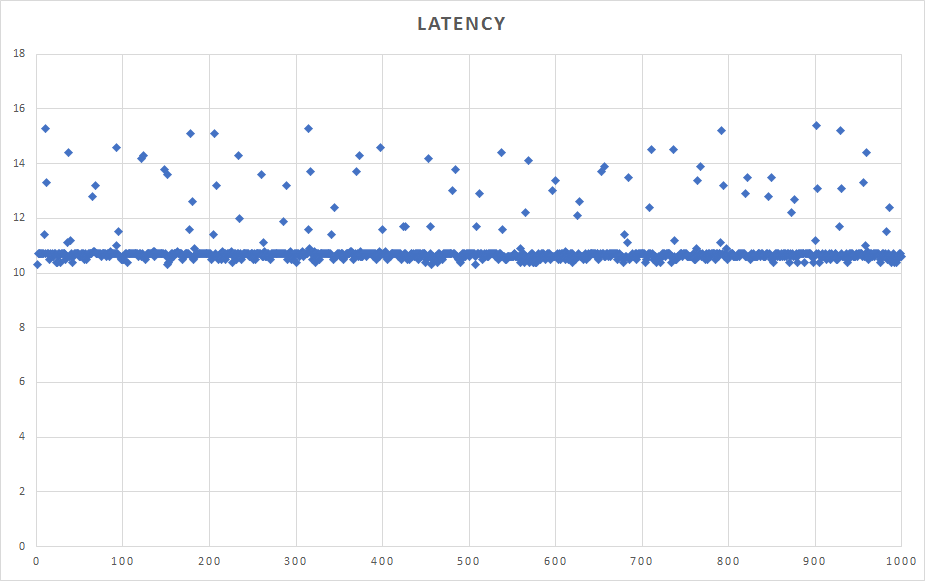
\includegraphics[scale=0.5]{Latency_Chart}
	\begin{figure}[h]
		\caption{Graph displaying the latency of 1000 ping packets}
	\end{figure}
\end{center}

As you can see from the graph, the actual latency is slightly more than 10 ms with the exact average being ``10.8337", this is around 7.7\% over the entered value of 10 ms. 
These results as mentioned previously were performed on the loopback address, this will simulate moving data over a network but with virtually perfect conditions, this therefore means that the extra time on top of the latency value is the overhead of processing the packet and issuing latency. One solution to this would be to incorporate more accurate time keeping mechanisms that will start a timer the second the packet is received and release it exactly when needed. With all things considered the accuracy of the simulated degradation is not one of the main objectives of the project, but will be incorporated as extra improvements later in the project if time allows.

\subsection{Testing effects}
The most effective way to visualise real world connections were running tests on SpeedTest.net \footnote{\url{http://beta.speedtest.net/}}. This is very useful to quickly visualise a certain effect on the network.

Below are two images showing the effect of a 100ms latency on a networks speed. Both tests were performed on the same empty network and the best result was taken from 5 runs on each.

\begin{center}
	
\includegraphics[scale=0.5]{SpeedNoEffect}
	\begin{figure}[h]
		\caption{The initial connection speed}
	\end{figure}
\end{center}

\begin{center}
	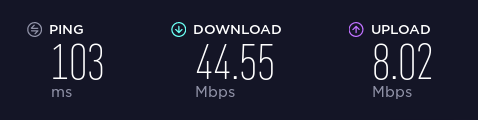
\includegraphics[scale=0.5]{Speed100ms}
	\begin{figure}[h]
		\caption{Network speed with a latency of 100m/s}
	\end{figure}
\end{center}

As you can see from both images, the 100ms has evidently been applied effectively and the speed of the connection has dropped by around 10Mbps. This means in real world terms the time taken to download a 1GB file would take 35 seconds longer to download. This is not a considerable reduction but the latency is having a obvious effect on the network quality.

Below are some graphs showing how the network speed deteriorates as the values of latency and packet loss rise:

\begin{center}
	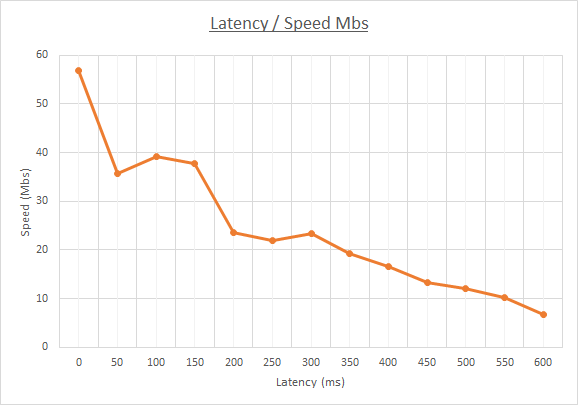
\includegraphics[scale=0.8]{Latency_Graph}
	\begin{figure}[h]
		\caption{Latency against download speed}
	\end{figure}
\end{center}

\begin{center}
	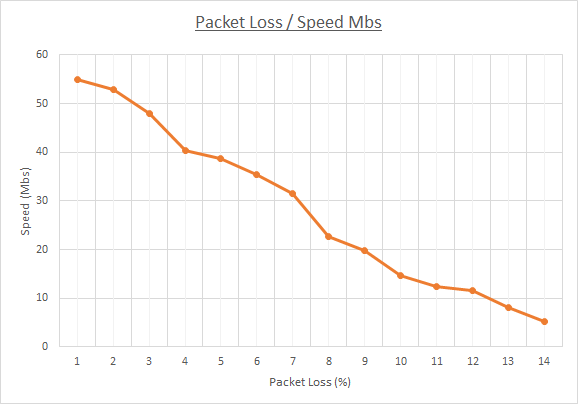
\includegraphics[scale=0.8]{PacketLoss_Graph}
	\begin{figure}[h]
		\caption{Packet loss against download speed}
	\end{figure}
\end{center}

As you can see from both graphs the more hostile the conditions the slower the connection. A general assumption from the graphs is that packet loss seems to be more consistent in effecting networking conditions, this could however be due to how accurately the packet loss is simulated with a more accurate representation thus giving more consistent results.

\section{Test Design}
There are various sections of the project that require a separate testing plan:

\begin{itemize}
\item Traffic simulation programs\\
These are the client server programs that will simulate traffic over the synthetic net. These tests will need to make 	sure each client and server performs its role correctly.
\item Packet script and effects\\
This is the script that will run on the custom router. Tests will be checking effects do their basic jobs and the script can be controlled effectively.
\end{itemize}

\subsection{Traffic simulation programs}
The test plan for this section will need to check all the intended functionality of each window. There are three aspects of each that will need testing:

\begin{itemize}
\item UI \\
Tests will be created that click buttons and check user interface works effectively through automated testing.

\item Business Logic \\
Code behind the UI will have the relevant methods testing with expected and actual results.

\item Real world usage \\
The involvement of multiple windows and more complex functionality can be tested by using automated testing scripts.
\end{itemize}

Appendix B contains the test plan for the programs, each separate program has had its user interface and business logic tested and programs that are to be used together have had ``Live" tests created to check their interaction together. The automated tests have been achieved by using the CUIT (Coded User Interface Tests) \footnote{\url{https://msdn.microsoft.com/en-us/library/dd286726.aspx}} that are built into Visual Studio 2017. These allow clicks and movements to be recorded and repeated.

\subsection{Packet Script}
It was decided that a separate test plan was needed for the script that will be run on the router. This was because its design is different to that of the traffic simulation programs. Each individual effect needs a basic test that uses a loopback ping test to simulate incoming traffic where a criteria is looked for, for example to test packet loss, the test pings the script until a packet is lost or a time-out is reached, this can perform a basic test on the functionality of the effect. Each effect will also require validation for the passed parameters, there will be a test created that will test various values inside and outside of the validation range.

At the end of Appendix B is the created test plan for the script. Due to the complexity of the script the test plan has remained short and therefore doesn't extensively test every possibility, this is due the initial unknown requirements of the script. This therefore was decided on a semi ad-hoc testing approach where the basic design of the tests would be added initially before implementation and later tests would be added where required.

\section{Testing methodology considerations}
Initially the methodology chosen to start development of the traffic simulation programs was "test driven development" \citep{beck2003test}, this was a tight methodology that increased development time but gave the added benefit of showing that new changes have not broken older functionality. This methodology was good to start off the project and allowed for a tight structure to be created where no time was wasted debugging previously working code, but as mentioned this methodology slowed development time down, this was chosen to be abandoned after 3-4 weeks to an ad-hoc approach. This was due to time restraints on the project and the less-important role that the traffic simulation programs has on the project compared to the degradation simulation script. The degradation script was developed in the ad-hoc approach, this was due to issue stated previously about the unknown aspects of the script and how it would be operating that it was decided that the time invested to write up scripts would assume too much and would risk them having the be completely rewritten, tests therefore are to be written on demand when new functionality has been included.


%================================================================================================================%
%Class Structure:
%This can include UML diagrams such as class diagrams, use case diagrams, activity diagrams, etc.
%If you find that these are taking up a lot of space/words, then you should prioritise and relegate where appropriate to the appendices. 
%This should not just be a list of unexplained diagrams, but should rather include discussions of the most interesting parts of your design, tying them to your background and objectives.
%
%UI design:
%If your software includes user interaction then you could also include a discussion (supported by diagrams) of decisions that you have made regarding the user interface.
%
%Experimental design:
%If you project includes any experiments, including but not limited to user testing, then you can discuss their design here. Note that again this does not exist in a vacuum and should be tied to your research.
%
%Test design:
%Testing is an extremely important part of any software project and should not be a tacked on afterthought. You can include here a discussion of the design of any tests that you intend to carry out on your project. It would not be appropriate to include an exhaustive list of all the individual tests that you wish to conduct (consider the appendices for this) but examples would be useful to illustrate your discussion.
